`\chapter{Literature Review}
	This literature review is split into two sections: one on traffic forecasting and the other on activity modeling.  This split was chosen due to its logical similarity to our approach.  It is first necessary to understand other forecasting techniques and then activity models which we will use to improve on the best forecasting technique.  The publications were chosen based on similarity to the work laid out in this paper, novelty of technique, and extent with which the methods described may be utilized in this work.  Taken together, they show a lack of research specific to using group activity modeling to improve forecasting performance in roadway or building environments.

\section{Traffic Prediction}

\subsection{Auto Regressive Moving Average Models}
Due to the importance of auto regressive moving average (ARMA) based models, specifically the seasonal auto regressive integrated moving average (ARIMA) model in this work, we briefly introduce such models in this section.  For a more detailed description of ARMA and seasonal ARIMA models refer to the textbooks by Box and Jenkins \cite{Box2008}, Franses \cite{Franses1998}, or Cryer and Chan \cite{Cryer2008}.  All notation for the models used below was taken from Box and Jenkins.

An ARMA model of with a number of $\phi$ and $\theta$ parameters, represented by p and q respectively is defined as: 
\begin{equation}
Y_{t} = \phi_{1}Y_{t-1} + \phi_{2}Y_{t-2} + ... + \phi_{p}Y_{t-p} + e_{t} - \theta_{1}e_{t-1} - \theta_{2}e_{t-2} - ... - \theta_{q}e_{t-q}
\end{equation}

\noindent
where $\{Y_{t}\}$ denotes the observed time series and $\{e_t\}$ represents an unobserved white noise series.  We abbreviate the model name to ARMA(p, q).  This approach involves training a set of parameters to fit a regression model based on a fixed number of historic readings.  ARMA based approaches are useful for their capability to predict further than one measured time instance in the future.    

For traffic data, many ARMA variations have been implemented such as ARIMA \cite{Williams2003}, VARMA \cite{Min2007}, STARMA \cite{Kamarianakis2003}, fractional ARIMA \cite{Xue1999}, and seasonal ARIMA \cite{Fillatre2003}.  Numerous papers \cite{VanDerVoort1996,Cho2003,Zhang2009,Taylor2006,Ishak2004} have been published comparing the results of ARMA based models vs other approaches.  While not always the best, ARMA models consistently forecast results on par with other state of the art approaches.  Another study \cite{Kamarianakis2003} compared univariate ARIMA models versus the multivariate STARIMA and VARIMA models.  On two datasets generated from the same road network over different times the univariate ARIMA was on par or slightly out performed multivariate models.  \newline

\textbf{Seasonal ARIMA}

Due to our traffic data having periodic trends and a non stationary mean, it is advantageous to use a seasonal ARIMA model.  An ARIMA model can handle non stationary means while periodic trends are handled by the seasonal component of the model.  The seasonal ARIMA model is defined as:
\begin{equation}
\label{eq:sarima}
\phi_{p}(B)\Phi_{p}(B^{s})\nabla^{d}\nabla^{D}_{s}z_{t} = \theta_{q}(B)\Theta_{Q}(B^{s})a_{t}
\end{equation}

\noindent
where B is the backshift operator, $a_{t} \sim N(0, \sigma^{2})$ is a white noise process, $\nabla^{i}_{j}$ is the seasonal difference operator, and $\phi,\  \Phi,\  \theta,\ \Theta$ are trainable parameters.  We represent seasonal ARIMA models as $ARIMA(p,d,q)(P,D,Q)_{s}$ where p is the number of autoregressive terms, d is the number of differences and q is the number of moving average terms.  P, D, and Q all correspond to the seasonal equivalents of p, d, and q.  The parameter $s$ is the seasonality of the model.\newline

\textbf{Additional motivation for using seasonal ARIMA models}

A source of error in seasonal ARIMA models is the presence of large infrequent transitory shocks \cite{Balke1994}.  In the context of seasonal ARIMA models a large shock value implies a large deviation from previous readings for the same time frame.  In the traffic domain this means that large shock values indicate the presence of large deviations in typical daily motion.  Recall that one of our assumptions is that there exists a set of discrete activities which account for much of the motion within the environment.  If these large deviations are one of these activities, then we would expect to see the seasonal ARIMA model forecast incorrectly in a consistent way.  

\begin{figure}[ht]
\begin{center}
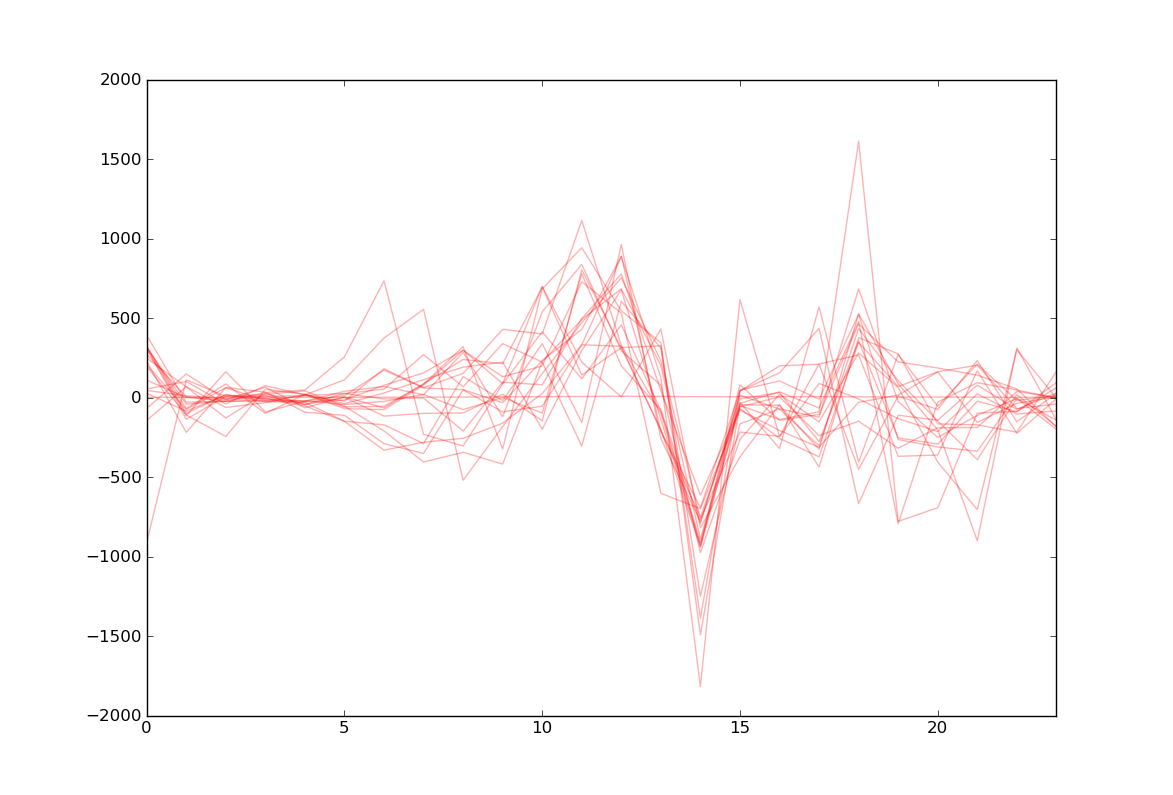
\includegraphics[width=0.8\textwidth]{broncos_residual.png}
\end{center}
\caption{Residual counts of all Broncos afternoon home games from 2008 - 2010}
\label{fig:broncos_residual}
\end{figure}

Empirically, we find that activities do produce semi-consistent errors in the forecasting of the seasonal ARIMA model.  Referencing the Broncos example again, figure ~\ref{fig:broncos_residual} shows the residual (actual observations - one step ahead seasonal ARIMA forecasts) counts of all Sunday afternoon Broncos from 2008-2010.  While there is some variance in the image, it is clear that the seasonal ARIMA model consistently incorrectly forecasts during the presence of a Broncos game.  This work looks to exploit such consistent incorrect forecasts by using residual data to train a set of activity models.

Despite the strong performance of ARMA based approaches to handle traffic forecasting, numerous other approaches are discussed below for a complete review of the literature.

\subsection{Other Approaches}
Neural networks offer another avenue for solving traffic prediction problems.  Such networks can be trained directly using a time series neural network, which is simply a network with additional input nodes to account for the past $m$ readings.  Research \cite{Taylor2006,Ishak2004} has shown performance to be generally comparable to Seasonal ARIMA models.  In one study neural networks performed better and in another seasonal ARIMA approaches performed better.  The actual performance is likely data dependent.

Due to their ease of implementation because of the abundance of available software packages and relatively low computation cost, neural networks seem to perform well in conjunction with other models.  \cite{Zheng2006} showed the feasibility of using multiple neural network models with final forecasts computed by a Bayesian combination of all other neural network models.  In another study \cite{Tseng2002} implemented a neural network based on the output of a seasonal ARIMA model.    In both studies, significant improvement to the MAPE for both training and test data were made with a combined approach as opposed to any singular model.  While not perfectly analogous, these approaches which utilize multiple models are similar to our activity based approach.

There has also been work into mapping traffic onto a graph structure which is a representation of the spatial layout of the environment\cite{Kriegel2008}.  Such work uses a statistical flow model to forecast the future density on any edge within the graph.  A graph approach has the benefit of improved forecasting on short time scales because it naturally limits the potential density of traffic of any edge based on the current state of the graph and how likely it is that one edge may affect another edge within a given amount of time.  To perform such forecasts, vehicles are assumed to drive along a shortest path to a set of possible destinations weighted by probability of ending at that destination.  When the forecast of future traffic density goes beyond the scale of a few time steps the number of possible destinations exponentially increases and as expected the future forecast error increases significantly.  This approach seems most promising for relatively short forecast time scales.  Also, this style of forecasting is not feasible if the data collection rate is relatively slow as at a certain collection rate there is no longer a strong correlation between the sensors within the network.

In an attempt to resolve the deficiencies in parametric models, such as ARMA, work has been done on non-parametric models.  In \cite{Smith2002,Zhang2009} a nearest neighbor approach was used where the state space was the last $n$ lag values, and forecasting was performed by aggregating the $k$ nearest neighbors values weighted by how recently the neighbor data was collected.  The idea is that when the data becomes too "chaotic" parametric models are unable to forecast.  Thus models which are not trained on pre-set parameters will be better able to account for such "chaotic" data.  In practice however, ARMA based models tend to out perform nearest neighbor approaches.  

\section{Individual Activity Modeling and Recognition}
Work in activity recognition has focused on recognizing either individual activities or group activities.  In this section we describe many of the individual activity recognition techniques.  One common type of individual activity recognition is from wearable sensors such as accelerometers or RFID tag readers.  This type of work is almost always supervised and the goal is to map sensor readings to a comprehensible activity such as dish washing or tooth brushing \cite{Wang2009,Bao2004}.  While some of this has potential applications to our goals, much of it is not applicable as the focus is typically on recognizing activities from fully labeled datasets.  Authors from this field have used many of the standard machine learning models: decision trees \cite{Bao2004}, support vector machines \cite{Krishnan2008,Bao2004,Lustrek2009}, naive Bayes \cite{Bao2004,Lustrek2009}, nearest neighbor \cite{Bao2004,Lustrek2009}, and hidden Markov Models (HMM) \cite{Wang2009,Oliver2002}.  Comparisons amongst models have shown that performance is data dependent and that no one model appears to be best for all types of activities \cite{Bao2004,Lustrek2009}

%Conditional random fields have been used as the basis for an activity \cite{Mahdaviani2007}.  Such a model has an advantage over hidden %Markov models used for the same task because is relaxes the observation independence assumptions that are inherent in such Markov %models.  Thus, the authors model activities as a sequence of conditionally dependent observations.  Also as a way to inhibit overtraining, a %entropy cost offset is used.

Huynh \cite{Huynh2008} used a naive Bayes classifier in a different way for wearable sensor individual activity recognition.  Instead of using it to describe activity, it was used as a dimensionality reduction technique the results of which were the basis for a dictionary in latent Dirichlet allocation \cite{Blei2003}.  The topics generated from latent Dirichlet allocation are then clustered using k-means.  Each of these clusters represents a single activity.  This clustering approach proved effective for the recognition of repeated activities throughout the day, but due to its reliance of a fixed ratio of latent Dirichlet allocation projected topics, it is likely that recognizing combinations of activities will prove problematic.

To account for activities of varying time lengths, probabilistic suffix trees \cite{Hamid2007} have shown to be an effective model for activities.  Trees are trained using all sequential subsets of an input sequence and a total model is then created from the set of trees using AdaBoost \cite{Freund1996}.  The performance level of suffix trees seems to be highly noise dependent.  \cite{Hamid2006} compared HMMs with suffix trees and found that suffix trees out performed HMMs when the data was without noise, but as the noise increased HMMs performed increasingly better, eventually surpassing the performance of suffix trees.


\section{Group Activity Modeling and Recognition}
There are a limited number of publications that exist on group activity modeling recognition using a large number of sensors.  Within this problem domain the challenges to solve are different due to the type of data collected and due to group activities typically occurring over multiple sensors.  The data from the sensors is normally binary which leads to ambiguity determining true counts and direction of motion for cars or people.  Despite this ambiguity it is relatively easy to automatically construct the topology of the sensors \cite{Wren2003, Wren2006a}.  Empirically it seems as though this topology roughly correlates to the spatial distribution of the sensors.  We will use this spatial information later to better model events which occur over multiple sensors.
	
HMMs have been used as a model for learned activities.  These models are used to build a tree \cite{Minnen2004, Wren2006a} with each level described by a model with a different number of hidden nodes meaning that model accuracy is roughly correlated to tree depth.  At the top of the tree are simple models used to describe gross activities.  The leaves of the tree are highly complex models describing specific activities.  This tree structure has the advantage of being computationally efficient while maintaining accuracy on par with other techniques based on clustering of HMMs \cite{Clarkson1999}.  
	
In a method similar to the HMM tree, work has been done to create a hierarchy of fixed filters based on possible sensor topologies \cite{Wren2006}.  At each level of the hierarchy, the number of sensors and the amount of time history increases.  The probability of occurrence of each fixed arrangement is then computed when all levels are created, the resulting model represents the total classifier.  The usage of fixed sensor topologies is highly environment dependent and the fixed time lengths with each level of the hierarchy are likely too restraining for the types of activities we expect to observe.  

From the results of all activity recognition papers, it appears that approaches which show the most promise tend to use a model which allows comparison of inputs with various time lengths.  Also, hierarchical techniques tend to perform better than multiple models of equal complexity.  In defense of these general observations is the work of Huynh \cite{Huynh2005} who found that empirically for his problem, there is not a single feature or time window of past history that will perform best for all activities.  Instead each activity is best modeled by a set of features and length of time unique to that activity.  Huynh postulates that his finding is true of most activity recognition problems and concludes that his finding demonstrates a fundamental flaw present in many of the activity recognition techniques to be described as the typical approach is to search for an optimal set of activity models for a fixed feature space and window of time.
